\documentclass[a4paper,11pt]{article}

\usepackage[utf8]{inputenc}
\usepackage{booktabs,tabularx, array, pdflscape}
\usepackage{geometry}
\usepackage{graphics,graphicx}
% \usepackage{subfigure}
\usepackage{subcaption}
\usepackage{color}
\usepackage{url}
\usepackage{enumerate}
\usepackage[table]{xcolor}
\usepackage{multirow}
%\usepackage{showframe}
\usepackage{adjustbox}

% \pagestyle{headings}

\setlength{\textheight}{24cm}  
\setlength{\textwidth}{15cm}
\setlength\oddsidemargin{0cm}
\setlength\evensidemargin{0cm}
\setlength\voffset{-1cm}

\renewcommand{\textfraction}{0.01}
\renewcommand{\floatpagefraction}{0.75}
\renewcommand{\topfraction}{0.8}
\renewcommand{\bottomfraction}{0.8}

\newcommand{\red}[1]{\textcolor{red}{#1}}	
\newcommand{\mc}[3]{\multicolumn{#1}{#2}{#3}}

\newcommand{\Ni}{({\em i\,})~}
\newcommand{\Nii}{({\em ii\,})~}
\newcommand{\Niii}{({\em iii\,})~}

%opening
\title{

\includegraphics[width=3cm]{./img/200px-SuitClubs.png} \\
\Huge M5.3 -- Final Evaluation
  \\ 
}
\author{\vspace*{1cm}\\ \LARGE Juliane Stiller$^1$, Vivien Petras$^1$ \& Andreas Lüschow$^2$ \medskip \\ \Large $^1$Humboldt-Universit\"at zu Berlin\\\Large $^2$Leibniz Institute for Psychology Information}
\date{\vspace*{2cm} -- v1.0 --\\September 2019}


\begin{document}

\clearpage\maketitle
\thispagestyle{empty}

\vspace*{5cm}
\begin{abstract}
This document presents the evaluation results from the CLUBS project. We describe the design of the evaluation experiment that allows us to compare the different systems that were developed. After presenting the outcomes (e.g., inter-annotator agreement) from a pilot experiment that was conducted before the final user evaluation, we give a detailed report about the different systems and their single evaluation results. The system that makes use of translated metadata performs best.
\end{abstract}

\newpage
\tableofcontents
\clearpage

% guarrada, no va el \cleardoublepage
% \clearpage\mbox{}\clearpage

%\newpage
\section{Introduction}
The project developed different approaches for Cross-lingual Information Retrieval (CLIR) using the use case of the PubPsych portal, a multilingual search engine in the psychological domain. The goal of the project was to define the technical approaches that have a positive impact on information retrieval performance and are suitable to offer retrieval across languages. The approaches tested implemented the following CLIR techniques:
\begin{itemize}
    \item query translation,
    \item content translation, and
    \item mapping of controlled vocabulary.
\end{itemize}
For evaluating the best approach and the performance of the best technique, we consider intrinsic and extrinsic evaluation (Fig.~\ref{fig:overview}). A detailed description of the evaluation plan for all approaches can be found in the relevant project documentation \cite{m1.3.1_2017}. 
%The results of the intrinsic evaluation of the different approaches for query translation and content translation with neural machine translation are described in \textcolor{red}{deliverable M5.1 ???}.

Furthermore, the project documentation in \cite{m1.3.2_2018} reports the single steps of the final retrieval performance test. The results of this final evaluation are detailed in the present report.
 
\begin{figure}[!hb]
\centering
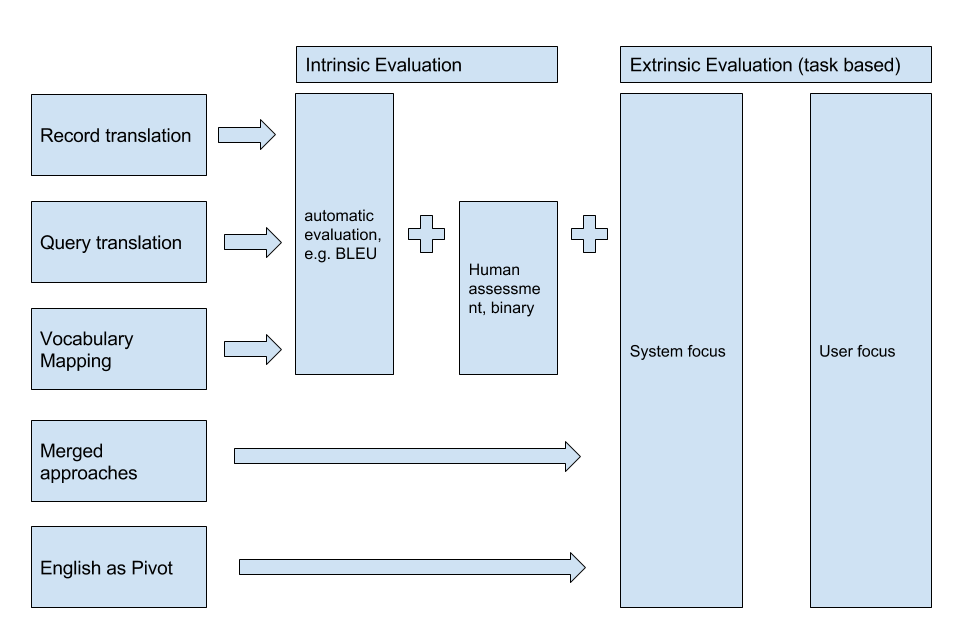
\includegraphics[width=14cm]{./img/overview_evaluation.png}
\caption{Plan for evaluation from the beginning of the project.}
\label{fig:overview}
\end{figure}

%%%%%
%%%%%
\newpage
\section{Design of Evaluation}
\subsection{Extrinsic system evaluation}
The extrinsic system evaluation assesses which of the implemented techniques for CLIR has the most positive impact on retrieval performance. For that, different systems that implemented solutions for CLIR are assessed. They are compared against a given baseline and with each other. 

\subsection{Design of experiment}
\label{sec:design_of_experiment}
To compare different systems that implemented the developed approaches, we establish a baseline for retrieval. This baseline is created using a selection of 50 original queries that were actually sent to PubPsych by real users, and their human translations into 4 languages, leading to 200 original queries in total. We query our baseline system and store the top 10 results for each query (Fig.~\ref{fig:queries}). Each other system is queried in the same way using these original queries. The systems have either content translation (i.e., machine translation of the search engine index) or real-time query translation implemented. 

\begin{figure}[!hb]
\centering
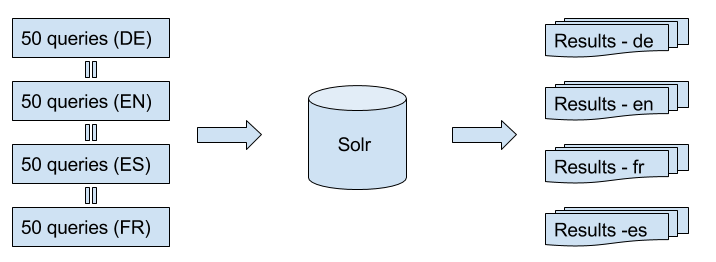
\includegraphics[width=14cm]{./img/queries.png}
\caption{Retrieving 200 results lists from a PubPsych system with 50 queries in 4 languages.}
\label{fig:queries}
\end{figure}

For each document found, the relevance in relation to the retrieving query is assessed by human judges. For that, we use topic descriptions written by domain experts that make the information need of the single queries explicit to the judges. In each tested system, we store up to ten results for each of the 200 searches (4 x 50 queries). If a query results in less than 10 results, we store all results for this query. 

After retrieving all documents, we remove duplicates (determined by the unique document ID and the topic they were retrieved with). The remaining documents are pooled by language of their metadata so they can be shown to a judge who understands this language. The judges assess the relevance of the document-query pairs on a three-point scale: highly, partially or non relevant. These relevance assessments allow us to compare results lists using the following measures ($r$ is the total number of relevant documents in the index found for a given query; all measures are calculated separately for each query and thus result list):

\begin{enumerate}
\item R-precision: If $r < 10$, we only look at the documents up to the $r$-th rank of the list. If $r >= 10$ then we calculate R-precision based on 10. In the latter case, values for R-precision and P@10 are identical.
\item P@10: We calculate the precision at 10 for the result list, i.e., the number of relevant documents on the first ten positions. As we only look at the first ten results, precision for the full result list will not be calculated separately.
\item Recall(10): How many of the relevant documents that exist for a query were actually found? If $r < 10$, recall is measured based on the actual number $r$. If $r >= 10$, the recall is measured based on $r = 10$ because only ten result documents will be looked at. In this case, Precision and Recall have identical values.
\item nDCG (normalized discounted cumulative gain): A rank-based measure. For this metric, the graded relevance (highly, partially, non relevant) of each document is important. Documents are weighted according to their graded relevance and their position on the result list. Hence, to achieve a high nDCG score, highly relevant documents must also occur high up in the ranked results lists.
\end{enumerate}
    
The assessment of the document-query pairs is conducted using \textit{CLUBS Compa}, a tool that was specifically developed during the project. Fig.~\ref{fig:tool} shows a screenshot of the tool with a document and its title, abstract, authors, and keywords in the middle of the screen. The retrieving query and the topic description are shown on the left side and the possible ratings judges can choose from on the right side. The tool has a user management system that automatically shows only those documents to a user which are written in the user's language. All ratings are saved in a database and can be exported for further analyses.

\begin{figure}[hb]
\centering
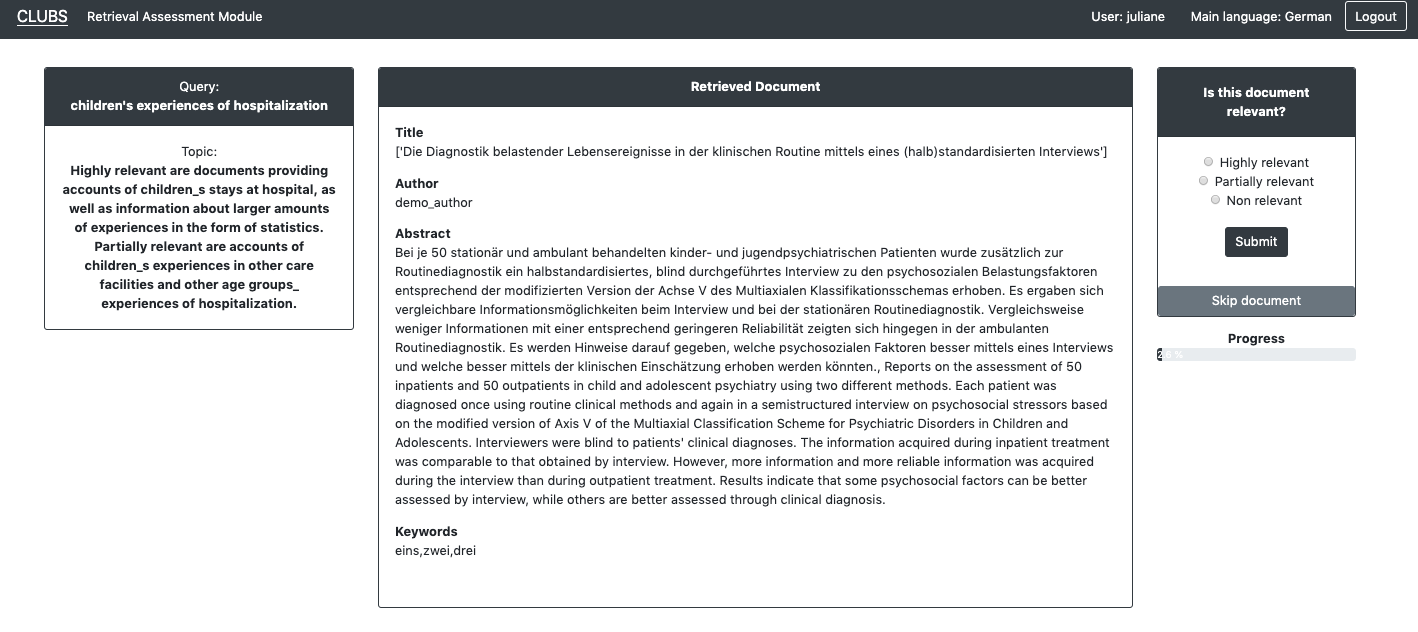
\includegraphics[width=14cm]{./img/screenshot_tool.png}
\caption{Tool used for rating the relevance of documents for a retrieving query.}
\label{fig:tool}
\end{figure}

%%%%%
%%%%%
\section{Pilot Experiment}
To test the experiment design as outlined above and in \cite{m1.3.2_2018} and the assessment tool as well as the topic descriptions, a pilot evaluation is set up. As the retrieval experiment is in a multilingual environment, we want to test and collect data in this pilot experiment with regard to the following points:

\begin{itemize}
    \item Get some mock first results.
    \item Estimate the time needed for the final evaluation.
    \item Identify problems with the topic descriptions.
    \item Which languages should the assessors speak? Do we need native speakers or can all assessors rate the English translations of the documents? To clarify this point, we calculate the inter-annotator agreement between different judges and see if the evaluation on the English translations of the documents is the same as the evaluation on the original documents. If the evaluation on English translations is as good as the evaluation on original content, we can only use English speaking assessors, which would probably be easier to acquire.
    \item Identify pain points that could be an issue for the real evaluation.
    \item Test the tool, its usability, database and document loading routine.
\end{itemize}

\subsection{Experiment set-up}
For the pilot assessment, we choose the set-up as outlined in Fig.~\ref{fig:experiment}. We use the 50 original queries in English to retrieve 100 documents in German, French and Spanish each. We extract these 300 documents from the results lists. We retrieve the same 300 documents in a system where the content was already translated into our four target languages to get these 300 documents also in English.  

As a French native speaker could not be recruited, only the 100 German and the 100 Spanish documents are rated. The 300 translated documents are rated twice, once by the German and once by the Spanish rater. This set-up allows to compare the ratings of a judge rating native documents and rating their English translations (intra-annotator agreement) as well as the ratings of both judges rating the English documents (inter-annotator agreement).

\begin{figure}[h]
\centering
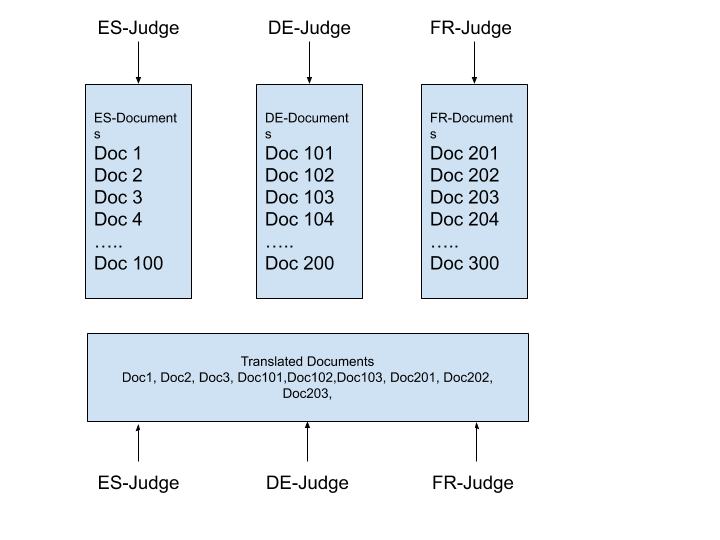
\includegraphics[width=10cm]{./img/IRpilotexperiment}
\caption{Experiment design for pilot evaluation with three judges. A French judge could not be recruited.}
\label{fig:experiment}
\end{figure}

\subsection{Results}
In total, 500 different documents were rated. 300 of these documents (the English ones) were rated twice, their original counterparts in German and in Spanish were rated once by each judge. Table~\ref{tab:pilot_matrix} shows the distribution of ratings for each rater. The ratings are not evenly distributed, there are far more ratings in the two \textit{relevant} categories (highly, partially) than in the \textit{non-relevant} category.

\begin{table}[h]
\centering
\begin{tabularx}{.73\textwidth}{lp{4cm}p{3.9cm}}
\addlinespace
\toprule
\ & \textbf{Rating} & \textbf{\# of documents} \\ 
\addlinespace
\cmidrule{1-3}
\addlinespace
\multirow{3}{*}{\textbf{Rater ES}} & Highly relevant & 207 \\
& Partially relevant & 127 \\
& Non relevant & 66 \\ 
\addlinespace
\multirow{3}{*}{\textbf{Rater DE}} & Highly relevant & 212 \\
& Partially relevant & 114\\
& Non relevant & 74\\ 
\addlinespace
\bottomrule
\end{tabularx}
\caption{Number of ratings per category and rater for 400 documents each.}
\label{tab:pilot_matrix}
\end{table}

\subsubsection{Intra-annotator agreement}
\label{subsec:intra}
The intra-annotator agreement shows the agreement between a single assessor rating documents in the assessor's native language---in our case German (Table~\ref{tab:pilotratDE}) or Spanish (Table~\ref{tab:pilotratES})---and the same documents in their English translation.

\begin{table}[h]
\centering
\begin{tabularx}{.7\textwidth}{llllll}
\addlinespace
\toprule
&&
\multicolumn{3}{c}{DE} \\ \addlinespace
\cmidrule{3-6}
\addlinespace
& & Highly & Partially & Non & total\\ \addlinespace
\cmidrule{3-6}
\addlinespace
\multirow{4}{*}{EN} & Highly & 43 & 11 & 0 & 54 \\
& Partially & 7 & 13 & 1 & 21 \\
& Non & 2 & 10 & 13 & 25 \\
& total & 52 & 34 & 14 & 100 \\
\addlinespace
\bottomrule
\end{tabularx}
\caption{Rating matrix for the original German documents and their English translations rated by the same judge.}
\label{tab:pilotratDE}
\end{table}

\begin{table}[h]
\centering
\begin{tabularx}{.7\textwidth}{llllll}
\addlinespace
\toprule
&&
\multicolumn{4}{c}{ES} \\ \addlinespace
\cmidrule{3-6}
\addlinespace
& & Highly & Partially & Non & total\\ \addlinespace
\cmidrule{3-6}
\addlinespace
\multirow{4}{*}{EN} & Highly & 44 & 5 & 3 & 52 \\
& Partially & 4 & 25 & 3 & 32 \\
& Non & 2 & 4 & 10 & 16 \\
& total & 50 & 34 & 16 & 100 \\
\addlinespace
\bottomrule
\end{tabularx}
\caption{Rating matrix for the original Spanish documents and their English translations rated by the same judge.}
\label{tab:pilotratES}
\end{table}

Of particular interest are the documents which were rated \textit{non-relevant} in one result set but \textit{highly relevant} in the other result set (German judge: 2 documents; Spanish judge: 2+3 documents). We analyze these documents to see if components of the experiment design need to be adapted. 

Intra-annotator agreement for each rater can be found in Table~\ref{tab:Intrapilot}. The measures are calculated for the rating of all three rating categories (highly, partially and non-relevant) as well as for only two categories where \textit{highly} and \textit{partially relevant} are considered to be a single \textit{relevant} category. 

\begin{table}[h]
\begin{tabularx}{\textwidth}{p{2cm}llll}
 \addlinespace
 \toprule
 \addlinespace
 &
 \multicolumn{2}{c}{Rater DE} &
 \multicolumn{2}{c}{Rater ES}\\
 \addlinespace
 \cmidrule{2-5}
 \addlinespace
 & Cohen’s Kappa & Scott’s Pi & Cohen’s Kappa & Scott’s Pi\\
\addlinespace
\cmidrule{2-5}
\addlinespace
3 categories & 0.494 & 0.488 & 0.653 & 0.653\\ 
\addlinespace
\cmidrule{1-5}
\addlinespace
2 categories & 0.594 & 0.586 & 0.554 & 0.554\\
\addlinespace
\bottomrule
\end{tabularx}
\caption{Intra-annotator agreement for the German and Spanish assessor.}
\label{tab:Intrapilot}
\end{table}

\subsubsection{Inter-annotator agreement}
\label{subsec:inter}
Inter-annotator agreement measures the agreement of ratings of the German and the Spanish rater. These measures are shown in Table~\ref{tab:Interpilot}. Both Tables~\ref{tab:Intrapilot} and \ref{tab:Interpilot} show Cohen's Kappa and Scotts Pi. According to Landis and Koch \cite{landis_koch}, the kappa for all categories can be interpreted as ranging from fair (0.21--0.40) and moderate (0.41--0.60) to  substantial (0.61--0.80) agreement. The same applies for Scott's Pi.

\begin{table}[h]
\begin{tabularx}{\textwidth}{p{2cm}llll}
 \addlinespace
 \toprule
 \addlinespace
 &
 \multicolumn{2}{c}{Translations from Spanish} &
 \multicolumn{2}{c}{Translations from German}\\
 \addlinespace
 \cmidrule{2-5}
 \addlinespace
 & Cohen’s Kappa & Scott’s Pi & Cohen’s Kappa & Scott’s Pi\\
\addlinespace
\cmidrule{2-5}
\addlinespace
3 categories & 0.556 & 0.554 & 0.502 & 0.494\\ 
\addlinespace
\cmidrule{1-5}
\addlinespace
2 categories & 0.702 & 0.702 & 0.664 & 0.664\\
\addlinespace
\bottomrule
\end{tabularx}
\caption{Inter-annotator agreement between the German and Spanish assessor.}
\label{tab:Interpilot}
\end{table}

\subsection{Limitation of experiment and learnings}
For the pilot experiment, we were not able to recruit a native French speaker that can rate the relevance of French documents. Therefore, we could not gain data for this particular language. We also set out to assess the effect of machine translation on the assessment of documents. For our sample, we could not observe a difference in assessment. 

The data is coming from the real-world database PubPsych which in its pure form is often bilingual, i.e., many documents already come with two or more languages in their metadata. Without a detailed language analysis of the metadata it is not possible to say for sure which languages are present in the data. For example, abstracts and titles are often translated by the source databases (e.g., Medline) that deliver their metadata to PubPsych and thus already copied into an index field (e.g., the title field). Attributing whether a particular rating was based on a machine translation or a manual translation was not feasible in practice. 

Therefore, we decide to show judges in the final retrieval performance experiment as much information as possible: we extract the language-specific information for abstracts, titles and keywords as well as possible English translations that come from the source databases. We will use six judges, i.e., two for each language (German, French, Spanish), that are domain experts in the psychological domain. Every assessor should be able to rate English documents.

Furthermore, both raters in the pilot experiment were not domain experts and do not have a background in Psychology. We find that this aspect is crucial for the final experiment as the assessments are very dependent on the domain expertise of the judges. Additionally, the task of relevance assessment is extremely hard and strenuous due to topics such as abuse, violence, sicknesses covered, the domain vocabulary used, and the nature of the abstracts with their very compressed information. 

In  the pilot experiment, we were able to assess 50 documents per hour and expect this amount to be also feasible in the final experiment.\footnote{For comparison, the assessment of pictures/short documents retrieved with queries in the cultural heritage domain is much faster. Raters can achieve numbers of up to 400 document assessments per hour.}

%%%%%
%%%%%
\section{Retrieval Assessment of CLIR Approaches}
This section describes the results of the retrieval assessment of the different systems that implemented CLIR techniques.
For evaluation, we compare three different systems with each other as well as their performance against the baseline (Fig.~\ref{fig:diffsystems}).

\begin{figure}[h]
\centering
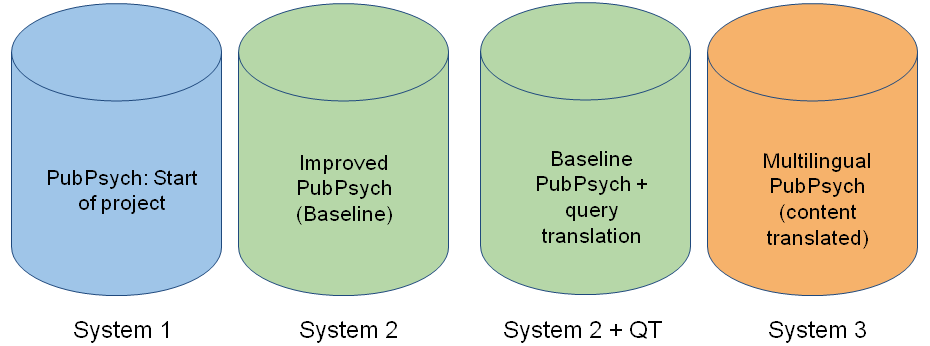
\includegraphics[width=14cm]{./img/systemseval}
\caption{Comparison of different systems in retrieval assessment.}
\label{fig:diffsystems}
\end{figure}

\subsection{The different systems evaluated}
The different systems that are evaluated:
\begin{itemize}
    \item \textbf{System 1:} This system is the unaltered system at the start of the project. It can serve as baseline system with regard to measuring the impact the project has as a whole on the performance of the system.
    \item \textbf{System 2:} This is considered to be the baseline system. This is an error free system which we set up after cleaning up the database of System 1 and introducing some changes to the search engine index and ranking algorithm.
    \item \textbf{System 2 with QT implemented:} This is the baseline system with an implementation of the query translation. All 200 queries (50 queries in 4 languages) are sent to this system and each query will be automatically expanded with translations into the other three languages.
    \item \textbf{System 3:} In this system, content in the PubPsych database is translated. Titles, abstracts and keywords are then available in English, German, French and Spanish. Thus, there is no need to additionally translate the query. All 200 original queries remain as they are.
    \item \textbf{System 3\_old:} This system works the same as System 3. However, the content translation is not based on the final machine translation (MT) system but on an old MT system. This older system was used in the pilot experiment and thus also needs to be used in the final evaluation to query the English documents for calculating inter-annotator agreement between the six judges (see also the explanations in Section~\ref{subsec:inter}).
\end{itemize}

To compare different approaches---e.g., human translated queries in System 2 against machine translated queries in System 2---different \textit{runs} are used to extract result lists from PubPsych. Table~\ref{tab:Runs} shows all these runs. Please note that the number of documents in this table does only represent the amount of documents in a run that were not yet part of one of the previous runs (i.e., duplicates are removed because they do not need to be rated again). In total, 3,304 documents need to be rated by the assessors; plus 100 documents for each judge for comparing the inter-annotator agreement with the pilot experiment.

\begin{table}[ht]
\adjustbox{max width=\textwidth}{
\begin{tabularx}{1.15\textwidth}{llllr}
%\toprule
\cmidrule{1-5}
\addlinespace
\textbf{System} & \textbf{Run name} &  \textbf{Queries} & \textbf{Translation} & \textbf{\# of docs}\\
\addlinespace
\cmidrule{1-5}
\addlinespace
System 1 & HT\_base &  200 original & - & 1259 \\ 
\addlinespace
System 2 & HT\_base8001 &  200 original & - & 192 \\ 
\addlinespace
System 2 & MT\_from\_DE\_base8001 &  150 MT & Queries with DE as source & 285 \\
\addlinespace
System 2 & MT\_from\_FR\_base8001 &  150 MT & Queries with FR as source & 253 \\
\addlinespace
System 2 & MT\_from\_ES\_base8001 &  150 MT & Queries with ES as source & 275 \\
\addlinespace
System 2 & MT\_from\_EN\_base8001 &  150 MT & Queries with EN as source & 146 \\
\addlinespace
System 2 + QT & MT\_combined\_base8001 &  
200 original & - & 159 \\ 
\addlinespace
System 3 & HT\_content\_trans &   200 original & content & 735 \\
\addlinespace
System 3\_old & pilot\_run &  - & -  & 100\\
\addlinespace
%\bottomrule
\cmidrule{1-5}
\end{tabularx}}
\caption{Overview of systems, runs and retrieved documents that need to be rated, excluding duplicates. MT = machine translated queries, HT = human translated (i.e., original) queries.}
\label{tab:Runs}
\end{table}


\subsection{System-focused evaluation}
The following subsections illustrate the compostition of result lists of the different runs. For each language the queries that retrieved results (i.e., result list length $>$ 0), the number of total retrieved documents, the number of retrieved documents in the top ten positions of the result ranking and the mean of retrieved documents is demonstrated.

\subsubsection{The baseline}
\paragraph{HT\_base.}
In the baseline there are 1,490 documents that need to be rated. Overall, the 50 queries in English, German, French and Spanish found 121,765 documents.

\begin{table}[h]
\centering
\begin{tabularx}{0.81\textwidth}{lllll}
\cmidrule{1-5}
\addlinespace
& \textbf{DE} & \textbf{EN} & \textbf{ES} & \textbf{FR} \\
\addlinespace
\cmidrule{1-5}
\addlinespace
Queries that retrieved results & 43 & 50 & 41 & 42 \\
Retrieved documents & 24,185 & 71,990 & 3,828 & 21,762 \\
Retrieved docs top ten & 366 & 500 & 277 & 347 \\
Mean of retrieved document (n=50) & 483.70 & 1439.80 & 76.56 & 435.24 \\
\addlinespace
\cmidrule{1-5}
\end{tabularx}
\label{result_list_analysis_base_8000}
\end{table}

\paragraph{HT\_base8001.}
Overall, the 200 original queries retrieved 118,978 documents. In the top ten results, 1,477 documents were retrieved.

\begin{table}[h]
\centering
\begin{tabularx}{0.81\textwidth}{lllll}
\cmidrule{1-5}
\addlinespace
& \textbf{DE} & \textbf{EN} & \textbf{ES} & \textbf{FR} \\
\addlinespace
\cmidrule{1-5}
\addlinespace
Queries that retrieved results & 42 & 50 & 38 & 42 \\
Retrieved documents & 23,714 & 69,971 & 3,817 & 21,476 \\
Retrieved docs top ten & 353 & 500 & 277 & 347 \\
Mean of retrieved document (n=50) & 474.28 & 1399.42 & 76.34 & 429.52 \\
\addlinespace
\cmidrule{1-5}
\end{tabularx}
\label{result_list_analysis_base_8001}
\end{table}

\subsubsection{Machine translated queries}
\paragraph{MT\_from\_EN\_base8001.}
Overall, the 150 from English translated queries retrieved 49,813 documents. In the top ten results, 799 documents were retrieved.

\begin{table}[h]
\centering
\begin{tabularx}{0.81\textwidth}{llll}
\cmidrule{1-4}
\addlinespace
& \textbf{DE} & \textbf{ES} & \textbf{FR} \\
\addlinespace
\cmidrule{1-4}
\addlinespace
Queries that retrieved results & 35 & 29 & 39 \\
Retrieved documents & 16,540 & 5,674 & 27,599 \\
Retrieved docs top ten & 262 & 211 & 326 \\
Mean of retrieved document (n=50) & 330.80 & 113.48 & 551.98 \\
\addlinespace
\cmidrule{1-4}
\end{tabularx}
\label{result_list_analysis_mt_en}
\end{table}

\newpage

\paragraph{MT\_from\_DE\_base8001.}
Overall, the 150 from German translated queries retrieved 79,273 documents. In the top ten results, 852 documents were retrieved.

\begin{table}[!h]
\centering
\begin{tabularx}{0.81\textwidth}{llll}
\cmidrule{1-4}
\addlinespace
& \textbf{EN} & \textbf{ES} & \textbf{FR} \\
\addlinespace
\cmidrule{1-4}
\addlinespace
Queries that retrieved results & 39 & 28 & 33 \\
Retrieved documents & 53,919 & 9,040 & 16,314 \\
Retrieved docs top ten & 364 & 210 & 278 \\
Mean of retrieved document (n=50) & 1078.38 & 180.80 & 326.28 \\
\addlinespace
\cmidrule{1-4}
\end{tabularx}
\label{result_list_analysis_mt_de}
\end{table}

\paragraph{MT\_from\_FR\_base8001.}
Overall, the 150 from French translated queries retrieved 62,631 documents. In the top ten results, 733 documents were retrieved.

\begin{table}[h]
\centering
\begin{tabularx}{0.81\textwidth}{llll}
\cmidrule{1-4}
\addlinespace
& \textbf{DE} & \textbf{EN} & \textbf{ES} \\
\addlinespace
\cmidrule{1-4}
\addlinespace
Queries that retrieved results & 25 & 37 & 26 \\
Retrieved documents & 12,789 & 44,992 & 4,850 \\
Retrieved docs top ten & 207 & 328 & 198 \\
Mean of retrieved document (n=50) & 255.78 & 899.84 & 97.0 \\
\addlinespace
\cmidrule{1-4}
\end{tabularx}
\label{result_list_analysis_mt_fr}
\end{table}

\paragraph{MT\_from\_ES\_base8001.}
Overall, the 150 from Spanish translated queries retrieved 115,097 documents. In the top ten results, 767 documents were retrieved.

\begin{table}[h]
\centering
\begin{tabularx}{0.81\textwidth}{llll}
\cmidrule{1-4}
\addlinespace
& \textbf{DE} & \textbf{EN} & \textbf{FR} \\
\addlinespace
\cmidrule{1-4}
\addlinespace
Queries that retrieved results & 24 & 37 & 32 \\
Retrieved documents & 25,731 & 51,228 & 38,138 \\
Retrieved docs top ten & 199 & 309 & 259 \\
Mean of retrieved document (n=50) & 514.62 & 1024.56 & 762.76 \\
\addlinespace
\cmidrule{1-4}
\end{tabularx}
\label{result_list_analysis_mt_es}
\end{table}

\subsubsection{Automatic query translation}
\paragraph{MT\_combined\_base8001.}
Overall, the 200 original queries retrieved 964,975 documents. In the top ten results, 1,635 documents were retrieved.

\begin{table}[h]
\centering
\begin{tabularx}{0.81\textwidth}{lllll}
\cmidrule{1-5}
\addlinespace
& \textbf{DE} & \textbf{EN} & \textbf{ES} & \textbf{FR} \\
\addlinespace
\cmidrule{1-5}
\addlinespace
Queries that retrieved results & 46 & 50 & 43 & 46 \\
Retrieved documents & 265,219 & 427,708 & 87,941 & 184,107 \\
Retrieved docs top ten & 392 & 500 & 350 & 393 \\
Mean of retrieved document (n=50) & 5304.38 & 8554.16 & 1758.82 & 3682.14 \\
\addlinespace
\cmidrule{1-5}
\end{tabularx}
\label{result_list_analysis_8004}
\end{table}

\newpage

\subsubsection{Content translation}
\paragraph{HT\_content\_trans.}
Overall, the 200 original queries retrieved 386,465 documents. In the top ten results, 1,910 documents were retrieved.

\begin{table}[!h]
\centering
\begin{tabularx}{0.81\textwidth}{lllll}
\cmidrule{1-5}
\addlinespace
& \textbf{DE} & \textbf{EN} & \textbf{ES} & \textbf{FR} \\
\addlinespace
\cmidrule{1-5}
\addlinespace
Queries that retrieved results & 47 & 50 & 48 & 50 \\
Retrieved documents & 63,862 & 142,070 & 80,415 & 100,118 \\
Retrieved docs top ten & 444 & 500 & 467 & 499 \\
Mean of retrieved document (n=50) & 1277.24 & 2841.40 & 1608.30 & 2002.36 \\
\addlinespace
\cmidrule{1-5}
\end{tabularx}
\label{result_list_analysis_8003}
\end{table}


\subsubsection{Interpretation}
The tables above allow for some further evaluation of the performance of the different systems. Table~\ref{tab:comparisons_runs} gives an overview of the comparisons we can do with the different runs.

\begin{table}[ht]
\adjustbox{max width=\textwidth}{
\begin{tabularx}{1.15\textwidth}{llll} 
\toprule
\addlinespace
Run A & Run B & Purpose \\ 
\addlinespace
\toprule
\addlinespace
HT\_base & HT\_base8001 & The effect of changes to the system (start of\\ & & project) to improvements \\ 
\addlinespace
HT\_base8001 & 
MT\_from\_XX\_base8001 & 
Effect of Machine Translation on Retrieval:\\
& & does a human translated query produce\\
& & better results than the MT one? \\ 
\addlinespace
HT\_base8001 & HT\_content\_trans & Effect of content translation on retrieval\\ 
& & compared to baseline\\
\addlinespace
HT\_base8001 & MT\_combined\_base8001 & Effect of query translation on retrieval\\ 
& & compared to baseline\\ 
\addlinespace
MT\_combined\_base8001 & HT\_content\_trans & 
Compare query vs. content translation\\ 
\addlinespace
% & & Compare baseline with query+content translation \\ 
\addlinespace
\bottomrule
\end{tabularx}}
\caption{Possible comparisons with the different runs.}
 \label{tab:comparisons_runs}
\end{table}

\begin{itemize}
    \item HT\_base vs.\ HT\_base8001: The latter does not find as much documents as the other one. Additionally, there are 4 more queries that do not find documents at all in the baseline system. This does not necessarily mean that the baseline system performs worse than before the start of the project---it is probable that the original system had some indexing and ranking errors that led to the retrieval of irrelevant documents. However, this assumption needs to be proven with the final evaluation metrics (see section~\ref{results}).
    \item HT\_base8001 vs.\ MT\_from\_XX\_base8001: All runs in which the queries were automatically translated from one of the four languages perform worse than the baseline system which uses human translated queries. They do by far not retrieve as much documents as the original queries and the number of queries with zero results increases notably.
    \item HT\_base8001 vs.\ HT\_content\_trans: The system with content translation retrieves more than three times as much documents than the baseline system (118,978 vs.\ 386,465). The number of queries with a zero result list length decreases from 28 to 5. The amount of retrieved German documents is more than twice as high (23,714 vs.\ 63,862), the amount of French documents is four times as high (21,476 vs.\ 100,118) and the number of Spanish documents increases by a factor of 21 (3,817 vs.\ 80,415). Even for the English language, the number of retrieved documents doubles (69,971 vs.\ 142,070).
    \item HT\_base8001 vs.\ MT\_combined\_base8001: In the system that implemented real-time query translation, the amount of queries with zero length result lists also decreases (from 28 to 15), but not as much as with System 3. Furthermore, there seem to be some queries with a lot of retrieved documents but also many queries that lead to a result list with less than ten entries, because the number of retrieved documents in the top ten positions is not as near to 500 (the optimal number) as in System 3.
    \item MT\_combined\_base8001 vs.\ HT\_content\_trans: The comparison of these two systems can be deviated from the two previous paragraphs.
\end{itemize}

Table~\ref{tab:grouped_by_language} (Appendix) shows the number of retrieved top ten documents per system, grouped by different document and query languages. The data illustrates that, although retrieving more documents in total, System 2 with online query translation does not perform better than System 3 which retrieves the most documents for most of the languages. 

It is worth noticing that System 2 with query translation seems to perform best when it comes to Spanish metadata, retrieving considerably more documents in this language than the other approaches (except in those cases where Spanish is already the language of the query). Documents in the same language as the query are the most retrieved with the two baseline systems. This fact indicates that all other systems include more documents in their result lists that do not have the same language as the query, i.e., that the cross-lingual retrieval works.



Table~\ref{comparison_all_systems} (Appendix) summarizes the main insights from the system-focused evaluation and allows for a direct comparison of the outocmes from the different approaches.






% \begin{figure}
% \centering
% \includegraphics[width=12cm,height=8cm]{figs/Lang_results_de.png}
% \end{figure}
% \begin{figure}
% \centering
% \includegraphics[width=12cm,height=8cm]{figs/Lang_results_en.png}
% \end{figure}
% \begin{figure}
% \centering
% \includegraphics[width=12cm,height=8cm]{figs/Lang_results_es.png}\\
% \end{figure}
% \begin{figure}
% \centering
% \includegraphics[width=12cm,height=8cm]{figs/Lang_results_fr.png}
% \end{figure}






\subsection{User-focused evaluation}
\label{results}
The relevance of all found documents was rated by the six judges. This allows us to calculate the metrics as described in Section~\ref{sec:design_of_experiment}. Since all 50 queries lead to more than 10 relevant results ($r = 10$), Precision@10, Recall and R-precision have identical values.

Table~\ref{tab:performance_mt_systems} shows the retrieval performance for the machine translated queries used in System 2. All measures are lower than those for the baseline system, which underlines the observations made during the system-focused evaluation. The baseline system and the other approaches are illustrated in Table~\ref{tab:performance_all_systems}.

\begin{table}[ht]
\centering
\begin{tabularx}{\textwidth}{lllll}
\toprule
\addlinespace
& \textbf{MT from DE} & \textbf{MT from EN} & \textbf{MT from FR} & \textbf{MT from ES} \\
\addlinespace
\cmidrule{1-5}
\addlinespace
R-Precision &  \textbf{0.637} & 0.519 & 0.570 & 0.566 \\
\addlinespace
P@10 & \textbf{0.637} & 0.519 & 0.570 & 0.566 \\
\addlinespace
Recall(10) & \textbf{0.637} & 0.519 & 0.570 & 0.566 \\
\addlinespace
nDCG & \textbf{0.565} & 0.504 & 0.497 & 0.554 \\
\addlinespace
\bottomrule
\end{tabularx}
\caption{Comparison of machine translations -- retrieval performance}
\label{tab:performance_mt_systems}
\end{table}

\begin{table}[ht]
\centering
\begin{tabularx}{\textwidth}{lllll}
\toprule
\addlinespace
& \textbf{System 1} & \textbf{System 2} & \textbf{System 2} & \textbf{System 3} \\
& \textbf{(initial system)} & \textbf{(improved system)} & \textbf{+ QT} & \\
\addlinespace
\cmidrule{1-5}
\addlinespace
R-Precision &  0.660 & 0.651 & 0.714 & \textbf{0.830} \\
\addlinespace
P@10 & 0.660 & 0.651 & 0.714 & \textbf{0.830} \\
\addlinespace
Recall(10) & 0.660 & 0.651 & 0.714 & \textbf{0.830} \\
\addlinespace
nDCG & 0.569 & 0.567 & 0.606 & \textbf{0.702} \\
\addlinespace
\bottomrule
\end{tabularx}
\caption{Comparison of all systems -- retrieval performance}
\label{tab:performance_all_systems}
\end{table}

The system performing best is System 3 which uses content translation and no query translation. System 2 (the baseline) does not perform better that System 1 before the start of the project. This reveals that the changes to the index and ranking algorithm we implemented at the beginning of the project had no effect on the retrieval performance. However, they were necessary to prepare the software for being able to implement Systems 2 and 3. 

Compared to the baseline, System 2 with online query translation leads to an appreciable improvement in retrieval quality. However, System 3 shows the best scores and in combination with the analysis in the previous section, this system is the clear winner of the evaluation.


\subsection{Inter-annotator agreement}
We calculated the inter-annotator agreement between the six judges using the same documents as in the pilot experiment. Results are presented in Tables~\ref{tab:matrix_iaa_final} and \ref{iaa_scores_final}.

\begin{table}[!h]
\centering
\begin{tabularx}{.73\textwidth}{lp{4cm}p{3.5cm}}
\toprule
\addlinespace
\ & \textbf{Rating} & \textbf{\# of documents} \\ 
\addlinespace
\cmidrule{1-3}
\addlinespace
\multirow{3}{*}{\textbf{Rater DE 1}} & Highly relevant & 66 \\
& Partially relevant & 24 \\
& Non relevant & 10 \\ 
\addlinespace
\multirow{3}{*}{\textbf{Rater DE 2}} & Highly relevant & 60 \\
& Partially relevant & 28\\
& Non relevant & 12\\ 
\addlinespace
\multirow{3}{*}{\textbf{Rater FR 1}} & Highly relevant & 58 \\
& Partially relevant & 28\\
& Non relevant & 14\\ 
\addlinespace
\multirow{3}{*}{\textbf{Rater FR 2}} & Highly relevant & 41 \\
& Partially relevant & 37\\
& Non relevant & 22\\ 
\addlinespace
\multirow{3}{*}{\textbf{Rater ES 1}} & Highly relevant & 67 \\
& Partially relevant & 29\\
& Non relevant & 4\\ 
\addlinespace
\multirow{3}{*}{\textbf{Rater ES 2}} & Highly relevant & 62 \\
& Partially relevant & 23\\
& Non relevant & 15\\ 
\addlinespace
\bottomrule
\end{tabularx}
\caption{Number of ratings per category and assessor for 100 documents each.}
\label{tab:matrix_iaa_final}
\end{table}

\begin{table}[ht]
\begin{subtable}{.54\linewidth}
\begin{tabular}{p{0.85cm}ccccc}
 \addlinespace
\toprule
 \addlinespace
 & DE 2 & FR 1 & FR 2 & ES 1 & ES 2 \\
\addlinespace
\cmidrule{1-6}
\addlinespace
DE 1 & 0.524 & 0.384 & 0.305 & 0.318 & 0.539 \\
\addlinespace
\cmidrule{1-6}
\addlinespace
DE 2 & - & 0.389 & 0.343 & 0.102 & 0.450\\
\addlinespace
\cmidrule{1-6}
\addlinespace
FR 1 & - & - & 0.347 & 0.161 & 0.369\\
\addlinespace
\cmidrule{1-6}
\addlinespace
FR 2 & - & - & - & 0.130 & 0.347\\
\addlinespace
\cmidrule{1-6}
\addlinespace
ES 1 & - & - & - & - & 0.199\\
\bottomrule
\end{tabular}
\caption{Cohen's Kappa, 3 categories}
\end{subtable}%
\begin{subtable}{.54\linewidth}
\begin{tabular}{p{0.85cm}ccccc}
 \addlinespace
 \toprule
 \addlinespace
& DE 2 & FR 1 & FR 2 & ES 1 & ES 2 \\
\addlinespace
\cmidrule{1-6}
\addlinespace
DE 1 & 0.522 & 0.382 & 0.277 & 0.316 & 0.538 \\
\addlinespace
\cmidrule{1-6}
\addlinespace
DE 2 & - & 0.389 & 0.328 & 0.097 & 0.449\\
\addlinespace
\cmidrule{1-6}
\addlinespace
FR 1 & - & - & 0.335 & 0.154 & 0.368\\
\addlinespace
\cmidrule{1-6}
\addlinespace
FR 2 & - & - & - & 0.090 & 0.328 \\
\addlinespace
\cmidrule{1-6}
\addlinespace
ES 1 & - & - & - & - & 0.192 \\
\bottomrule
\end{tabular}
\caption{Scott's Pi, 3 categories}
\end{subtable}

\begin{subtable}{.54\textwidth}
\begin{tabular}{p{0.85cm}ccccc}
 \addlinespace
 \toprule
 \addlinespace
 & DE 2 & FR 1 & FR 2 & ES 1 & ES 2\\
\addlinespace
\cmidrule{1-6}
\addlinespace
DE 1 & 0.592 & 0.434 & 0.275 & 0.242 & 0.591\\
\addlinespace
\cmidrule{1-6}
\addlinespace
DE 2 & - & 0.293 & 0.443 & 0.202 & 0.615\\
\addlinespace
\cmidrule{1-6}
\addlinespace
FR 1 & - & - & 0.397 & 0.171 & 0.395\\
\addlinespace
\cmidrule{1-6}
\addlinespace
FR 2 & - & - & - & 0.175 & 0.507\\
\addlinespace
\cmidrule{1-6}
\addlinespace
ES 1 & - & - & - & - & 0.157\\
\bottomrule
\end{tabular}
\caption{Cohen's Kappa, 2 categories}
\end{subtable}%
\begin{subtable}{.54\textwidth}
\begin{tabular}{p{0.85cm}ccccc}
 \addlinespace
 \toprule
 \addlinespace
 & DE 2 & FR 1 & FR 2 & ES 1 & ES 2\\
\addlinespace
\cmidrule{1-6}
\addlinespace
DE 1 & 0.591 & 0.432 & 0.256 & 0.232 & 0.589 \\
\addlinespace
\cmidrule{1-6}
\addlinespace
DE 2 & - & 0.293 & 0.433 & 0.185 & 0.615\\
\addlinespace
\cmidrule{1-6}
\addlinespace
FR 1 & - & - & 0.390 & 0.145 & 0.395\\
\addlinespace
\cmidrule{1-6}
\addlinespace
FR 2 & - & - & - & 0.116 & 0.503 \\
\addlinespace
\cmidrule{1-6}
\addlinespace
ES 1 & - & - & - & - & 0.128 \\
\bottomrule
\end{tabular}
\caption{Scott's Pi, 2 categories}
\end{subtable}
\caption{Inter-annotator agreement in the final evaluation.}
\label{iaa_scores_final}
\end{table}

Some judges achieve a moderate agreement (0.41--0.60), most agreements are fair (0.21--0.40). Especially one of the Spanish assessors has rather bad agreements with the other judges. This may indicate a systematic error that was introduced into the experiment.

%%%%%
%%%%%
\section{Discussion}
In this section, we discuss the results of the previously described final project evaluation.

\subsection{System 2}
The baseline system with improved algorithm and indexing does overall perform equivalent to System 1 without adaptations. Most of the improvements were however necessary to make the search engine software more adaptable and to update the source code, so that the different implementations for this project could be integrated into the PubPsych system.

As Table~\ref{tab:grouped_by_language} shows, documents in the same language as the query are the most retrieved with the two baseline systems. This indicates that the implementations during the CLUBS project indeed improved multilingual retrieval, because more documents in other languages than the query language are retrieved in these systems. However, it needs to be examined to which extent such a "replacement" of documents in query language in favour of multilingual content is accepted by search engine users. If they retrieve a document whose metadata is translated but where they can not read the original document, such a document may be considered irrelevant even if the ranking algorithm places it at the top of the result list.

\subsection{System 2 with query translation}
This system performs better than the baselines but not as good as the winning approach, System 3, albeit it retrieves a lot of documents that do not seem to be relevant. In fact, some of the queries generate very large result lists whereas other queries do not find anything at all. This is probably due to the online query translation that looks up words from the search query in a multilingual lexicon. 

If a query can not be found in this lexicon, its single words (tokens) are looked up in the dictionary.\footnote{For more information on how the online query translation approach works, see also the project documentation in \cite{m1.5_2018} and the relevant CLUBS article from MTSR 2018 conference \cite{espana_mtsr}.} Obviously, this leads to translations that are quite general and thus retrieve many documents. Additionally, the combination of search terms using the Boolean OR operator enlarges the number of potentially relevant documents. If one of the search terms is a preposition such as "of", "in" or "at", a translation of this term into three other languages also dilates the search result list. This may explain the high number of documents found with this approach.

\subsection{System 3}
This is the winner system. Both the system-focused evaluation of the result lists and the user-focused evaluation (i.e., relevance ratings) show a clear preference for this approach. This system will be integrated into PubPsych's live system and allows future users to make use of the cross-lingual features that were developed and evaluated during this project. 

As a next step, it will be necessary to implement the machine translation pipeline into PubPsych's indexing workflow to be able to translate document metadata as soon as it enters the index. The required scripts and translation models were developed during the project and can be reused. 










\addcontentsline{toc}{section}{References}
\bibliographystyle{plain}
\bibliography{references}

\newpage
\appendix
\section{Additional Tables}

\begin{table}[ht]
    \centering
    \begin{tabularx}{0.81\textwidth}{llllll}
\addlinespace
\toprule
\addlinespace
Query & Document & System 1 & System 2 & System 2 & System 3 \\
language & language & & & with QT & \\
\addlinespace
\cmidrule{1-6}
\addlinespace
DE & English & 75 & 65 & 96 & \textbf{172}  \\
\addlinespace
& French & 4 & 4 & \textbf{18} & 11 \\
\addlinespace
& German & \textbf{284} & 280 & 215 & 254 \\
\addlinespace
& Spanish & 2 & 4 & \textbf{63} & 5 \\
\addlinespace
& Missing / & 1 & 0 & 0 & 2 \\
& other & & & & \\
\addlinespace
EN & English & 393 & \textbf{414} & 283 & 351 \\
\addlinespace
& French & 9 & 9 & \textbf{35} & 16 \\
\addlinespace
& German & 94 & 68 & 81 & \textbf{117} \\
\addlinespace
& Spanish & 2 & 4 & \textbf{94} & 10 \\
\addlinespace
& Missing / & 2 & 5 & 7 & 6 \\
& other & & & & \\
\addlinespace
FR & English & 147 & 153 & 178 & \textbf{300} \\
\addlinespace
& French & \textbf{157} & 155 & 103 & 110 \\
\addlinespace
& German & 39 & 34 & 43 & \textbf{73} \\
\addlinespace
& Spanish & 1 & 3 & \textbf{67} & 11 \\
\addlinespace
& Missing / & 3 & 2 & 2 & 5 \\
&  other &&&& \\
\addlinespace
ES & English & 80 & 81 & 134 & \textbf{225} \\
\addlinespace
& French & 4 & 3 & 19 & \textbf{22} \\
\addlinespace
& German & 27 & 19 & 39 & \textbf{55} \\
\addlinespace
& Spanish & 161 & \textbf{169} & 152 & 158 \\
\addlinespace
& Missing / & 5 & 5 & 6 & 7 \\
& other &&&& \\
\addlinespace
\bottomrule
\end{tabularx}
\caption{Retrieved document languages in the four systems, grouped by query language.}
\label{tab:grouped_by_language}
\end{table}

\begin{table}[ht]
\centering
\begin{tabularx}{\textwidth}{lllll}
\toprule
\addlinespace
& \textbf{System 1} & \textbf{System 2} & \textbf{System 2 + QT} & \textbf{System 3} \\
& \textbf{(initial} & \textbf{(improved} &  &  \\
& \textbf{system)}  & \textbf{system)} & & \\
\addlinespace
\cmidrule{1-5}
\addlinespace
\# of queries & 24 & 28 & 15 & 5
 \\
with 0 results & & & & \\
out of 200 & & & & \\
\addlinespace
Sum of found & 121,765 & 118,978 & 964,975 & 386,465
 \\
documents for & & & & \\
queries & & & & \\
\addlinespace
Per language & De = 24,185 & De = 23,714 & De = 265,219 & De = 63,862\\
DE / EN & En = 71,990 & En = 69,971 & En = 427,708 & En = 142,070 \\
/ ES / FR & Es = 3,828 & Es = 3,817 & Es = 87,941 & Es = 80,415 \\
& Fr = 21,762 & Fr = 21,476 & Fr = 184,107 & Fr = 100,118 \\
\addlinespace
\# of documents & 1,490 & 1,477 & 1,635 & 1,910 \\
in top ten & & & & \\
\addlinespace
Mean of retrieved & De = 483.70 & De = 474.28 & De = 5304.38 & De = 1277.24 \\
documents across & En = 1439.80 & En = 1399.42 & En = 8554.16 & En = 2841.40 \\
queries (n=50)  & ES = 76.56 & ES = 76.34 & Es = 1758.82 & Es = 1608.30 \\
per language & Fr = 435.24 & Fr = 429.52 & Fr = 3682.14 & Fr = 2002.36 \\ 
\addlinespace
\addlinespace
\bottomrule
\end{tabularx}
\caption{Comparison of all systems -- describing statistics.}
\label{comparison_all_systems}
\end{table}

\end{document}
